\documentclass[Bachelorarbeit.tex]{subfiles}
\begin{document}

\graphicspath{{./figures/implementation/}}	%specifying the folder for the figures

\chapter{Implementation}
\label{ch:implementation}

For this thesis a software was written to be able to investigate the behaviour and results of the different types of networks and get visual and numerical results to be embedded in this written text. In this chapter the implementation-details of the software are discussed.

\section{Requirements}
The author of this thesis had access to the software of \cite{Breuer2015} which was written in C++ therefore the question is why a new software had to be written and why not the original could be used. The reason for it was that the original software supported only a very narrow feature-set focusing only on the numerical results of a fully-connected network. Thus a complete redevelopment in Java was the option used. The following requirements were identified:

\begin{itemize}
\item Java based.
\item Comprehensive GUI functionality.
\item Emulate the functionality of \cite{Breuer2015} and its results.
\item Represent arbitrary networks in the simulation.
\item Step-through forward and backwards in a simulation-run.
\item Run replications of simulations.
\item Store results of replications to be opened again for later usage.
\item Command-line mode to run previously defined number of replications.
\end{itemize}

\paragraph{Java based}
The original software was written in C++ which offers very much power and highest speed if used correctly but comes with a very high responsibility regarding memory-management. Java offers a much more relaxed programming model regarding memory-management as it is garbage collected. This does not mean that the programmer can waste memory without giving thought to it but that not as many aufwand into it. debugging is easier.
The most compelling argument for Java are the vast libraries which are included in the JDK which are missing in standard C++. As complete GUI-functionality for the whole software is a requirement Java is the way to go. Although multi-purpose libraries like Boost and GUI-frameworks like Qt are available for C++ too, it takes quite some time to set them up correctly for the target platform one develops for which implies that in C++ the development would always have been for just one platform whereas Java runs on every platform - if not platform-dependent stuff was used - without recompilation. As one will see later in the "Command-line mode"-Feature this is a major requirement to make this feature practical. Thus the reasons for using Java were:

\begin{itemize}
\item Platform-independence which applies to 3rd party libraries too.
\item GUI-framework provided by JDK.
\item Relaxed memory-management which emphasises fast iterations and easy debugging.
\item Support for smooth XML-Serialization.
\item 3rd party libraries for network-modelling and -visualization.
\end{itemize}

\paragraph{GUI functionality}
All functionality should be accessible through a GUI where some features e.g. "Inspection" are only possible to use through a GUI.

\paragraph{Emulate \cite{Breuer2015} functionality}
Of course the whole software should be a super-set of the functionality of the one found in \cite{Breuer2015} so this was the point to start from.

\paragraph{Arbitrary networks}
It should be possible to restrict trading between the agents to arbitrary networks. As network-modelling and -visualization library JUNG is used.

\paragraph{Step-through simulation}
The software should support to go through a simulation-run step-by-step and storing all steps of the simulation to jump back and forth between steps.

\paragraph{Real-time visualisation and information}
The original C++ software didn't provide real-time information about the current wealth-distribution and market-dynamics and provided the user just with the numerical results in the end through the means of a command-line output. For better understanding of dynamics of both wealth and markets a real-time visualisation of both are necessary together with extensive information on the current state like the offering-book, agent-information, network-activity, history of matches and the current equilibrium. Also the real-time visualisation is necessary to provide this written part of the thesis with diagrams of various results and processes.

\paragraph{Replications}
Because the whole trading-process includes randomness the results are subject to noise thus replications are an absolute must-have feature to be able to give reliable results. Each replications is independent from all others thus it is a candidate for parallel programming to speed up the already very time-consuming process of running replications. According to the number of CPU-cores the software should spawn threads up to the number of cores and run replications in parallel thus speeding up by a considerable amount of time.

\paragraph{Store results}
When running a bunch of replications for a given set-up the results of it should be automatically stored as XML to be accessible for later inspection thus conserving state and eliminating the necessity to re-run time-consuming simulation-runs with a high number of replications.

\paragraph{Command-line mode}
As already described replications are required to be implemented for parallel processing where up to the number of CPU-cores replications can run in parallel. When running a vast number of replications one does not need to GUI-functionality and most probably the machine is so occupied by the heavy work-load that a fließender usage of GUI would be not possible any-more. Thus replications should be runnable through a separate command-line mode of the thesis-software which reads information from a XML-File in which one can specify multiple simulation set-ups for which replications should be run. The command-line mode iterates through all configurations and runs the required replications and writes the result out for a later inspection. Obviously the more CPU-cores the faster a simulation-run with e.g. 50 replications finishes. For this reason most of the final replication-runs were done on a 40-core machine of the FH Vorarlberg which runs on Linux on which the thesis-software could be run easily because of Java's platform-independence.

\section{Functionality}
In this section the functionality of the thesis-software is explained to get an understanding of the implemented features.

\subsection{Emulate \cite{Breuer2015} functionality}
TODO markets, bp, abm, equilibrium. not: abbruchbedingung is different, more strict

\subsection{Inspection}
TODO step-by-step and matching-history

\subsection{Replications}
TODO 

\subsection{Experiments}
TODO results öffnen
experimente per xml definieren
über command-line laufen lassen

\section{Architecture}
In this section the basic architecture of the thesis-software is discussed. It is important to note that this thesis is a fat-client and has its major emphasis not on the software-development aspect but on the visual- and numerical results where the accompanying software is just a tool for the means to calculate theses required results. Thus the architecture is guided by a simple division of layers into front-end, controller and back-end. The front-end is responsible for input and output of the user through GUI or command-line. The controller-layer provides encapsulated chunks of functionality of the back-end to the front-end. It is necessary to abstract, encapsulate and combine the stateful nature of communication with the back-end into a separate layer instead of polluting the front-end with it and creating unnecessary dependencies. The back-end layer provides the functionality where the real work is done e.g. simulation is executed.
\medskip
Theoretically the dependencies are top-down where the front-end includes only controller-functionality, the controller includes only back-end functionality and the back-end has no dependencies to the preceding layers. In this thesis-software a more pragmatic approach was chosen so this dogma was not followed where over-engineering and over-complication would have resulted when sticking strictly to the separation of dependencies. Thus in very few cases the controller- and back-end layer include front-end layer functionality to create different types of network topologies in a more convenient way. Also the front-end accesses instances of pure back-end classes for graphical visualisation and information purposes. Despite the seemingly flawed architecture the development-process has proven to be very smooth and expansions and refactorings went quite smoothly and always resulted in a better and clearer structure with reduced code-smell which is always a sign for a good architecture.

\begin{figure}[H]
	\centering
  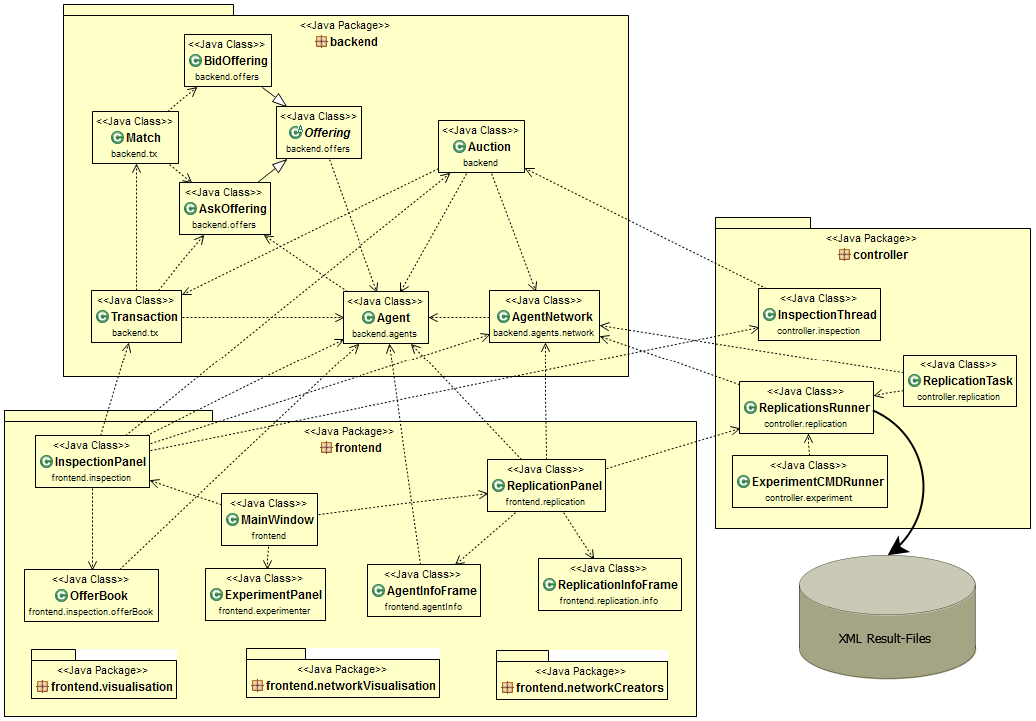
\includegraphics[width=1.0\textwidth, angle=0]{PACKAGE_DIAGRAM_MINIMAL.png}
	\caption{Package-diagram with most important classes and associations illustrating the architecture. (Note that the software contains many more classes and associations which are omitted for clarity reasons as this diagram should provide only a basic overview and would contain by far too much information if everything would have been included.)}
	\label{fig:PACKAGE_DIAGRAM_MINIMAL}
\end{figure}

\subsection{Frontend}
The front-end contains the GUI functionality through which the user interacts with the program and the real-time visualisation of wealth-distribution and market-activity. Because data like the offer-book, agent/replication/equilibrium-information and network-visualization is required in different contexts much emphasis was put on massive re-use of GUI components through the use of sub-classing and aggregation already provided by SWING. Thus many small components were implemented and aggregated together to create bigger chunks of logical functionality. In the package-diagram \ref{fig:PACKAGE_DIAGRAM_MINIMAL} only the most important panels are shown. Those provide the main entry-point for the user to the given functionality as indicated by their names.

\subsection{Controller}
The controller package is rather slim and contains the steering functionality to drive inspections, replications and experiments. Inspections are driven by the class \textit{InspectionThread} which allows to advance the simulation step-by-step using the consumer-producer paradigm through lock and wait functionality provided by Java through the use of its monitors. The classes \textit{ReplicationsRunner} and \textit{ReplicationTask} encapsulate functionality to run a number of replications for a given simulation-configuration in parallel, calculating the current median for all important values on-line and writing results to xml-files. Experiments are executed through the use of the class \textit{ExperimentCMDRunner} where it cycles through all simulation-configurations of a experiment-configuration and uses \textit{ReplicationsRunner} to execute it in parallel. 

\subsection{Backend}
The back-end contains the domain-specific functionality for the simulation. The important classes can be seen in the package-diagram \ref{fig:PACKAGE_DIAGRAM_MINIMAL} but for better clarity each one is introduced briefly.

\begin{itemize}
\item Auction - holds the state and operations for a single simulation-run. This class does the sweeping and clearing discussed in section "Simulation", determines whether trading is still possible or not and calculates current equilibrium.  allows to run a matching-round
\item Agent - encapsulates the functionality and state necessary for the agents in the simulation. See next section "Agents" for a more in-depth discussion.
\item AgentNetwork - holds the connections between the agents and provides functionality to query neighbourhood, paths and connections between agents and random and sequential in-order iterator over all agents.
\item Offering - encapsulates the data necessary for offerings where there are two subclasses \textit{BidOffering} and \textit{AskOffering} to differentiate between the two types of offerings. See the section "Markets" on details of offerings.
\item Match - provides the functionality to create a match out of given offers and returning an instance of \textit{Match} through a factory-method. The \textit{Match} instance holds the price, amount and the offers which have matched. See section "Sweeping and Matching" on more details.
\item Transaction - encapsulates functionality to search for a match within a given neighbourhood, is used by \textit{Auction} class to sweep through the agents and is returned after a matching-round and provides necessary information about whether it was successful or not.
\end{itemize}

\section{Agents}
Although agents are used in this software it is not an agent-based simulation in the classical way as these agents are zero-intelligence ones and have no states of behaviour. That is each agent makes bid- and ask-offers on all markets if the constraints allow it where the prices are selected from random ranges which improve the utility of the agent - that means it makes always offers which would result in a profit.

\medskip

Each agent is characterized by its state where the main variables are:

\begin{itemize}
\item Id - the unique id of the agent in the range of the natural numbers in the range of [1..number of agents].
\item Optimism-factor \textit{h} - defines how optimistic the agent is in the range of [0..1] where 0 is most pessimistic and 1 is most optimistic. The distribution of the optimism-factor among the agents is linearly ascending with the id and is defined through the following equation: \linebreak $\textit{optimism-factor} = \frac{id}{\textit{number of agents} + 1}$
\item Cash holdings - the current cash holdings of the agent.
\item Assets holdings - the current asset holdings of the agent not including the assets granted as securities for giving loans.
\item Loan given - the amount of loans bought from / granted to other agents. For a given amount of loans the equal amount of assets are granted as security to the buyer of the loan. Thus this variable increases the amount of assets the agent can trade with.
\item Loan taken - the amount of loans sold to other agents. For a given amount of loans the equal amount of assets the equal amount of assets are granted as security to the buyer of the loan. Thus this variable decreases the amount of assets the agent can trade with as this amount of loans needs to be kept as securities.
\end{itemize}

\medskip

There are three important derived variables which are calculated from the previous ones:

\begin{itemize}
\item Collateralized assets - is the amount of assets which are bound through collateral obligations because of taken bonds. \linebreak $\textit{collateralized assets} = max( 0, \textit{loans taken} - \textit{loans given} )$
\item Free assets - is the amount of assets which are unbound and act not as security and are owned completely by the agent. \linebreak $\textit{free assets} = \textit{Assets holding} - \textit{Collateralized assets}$
\item Loans - is the net number of loans and calculated through $\textit{loans} = \textit{loans given} - \textit{loans taken}$. Thus this value is positive if the agent has granted more loans to other agents than received and it is negative if the agent has received more loans from other agents than granted.
\end{itemize}

Note that all variables cannot go negative except loans.

\section{Markets}
In this section all markets and their implementations are described. Each market is completely characterised by the following points:

\begin{itemize}
\item Products - the products traded on the corresponding market.
\item Price-ranges - the price-ranges in which an agent places profit-making offers on the market.
\item Bid- and Ask-Offerings - define the pre-conditions for an agent to make offerings on the market and the amount and the prices generated during an offer. \medskip
Note that in case of bid-offerings the price of the profit-making offer is drawn randomly between the minimum price and the limit-price because when buying one wants to buy below the expected value to make a profit where in case of ask-offerings the price is drawn randomly between the limit-price and maximum price because when selling one wants to sell above the expected value to make a profit.
\item Match-Table - In case of a match between two agents the wealth-exchange is declared where the wealth is increased/decreased as indicated by the +/- signs.
\end{itemize}

\subsection{Asset/Cash}
\subsubsection{Products}
Free assets are traded against cash. The buyer gets a specific amount of free assets for a given amount of cash where the seller gives away the specific amount of free assets and gets the given amount of cash.

\subsubsection{Price-Range}

\paragraph{minimum}
The minimum value of one asset in cash is the down-value pD tomorrow as defined in chapter \ref{ch:leverageCycle} "The Leverage Cycle". This value is obviously a constant for all agents.

\begin{center}
$\textit{min asset-price} = \textit{pD}$
\end{center}
 
\paragraph{maximum}
The maximum value of one asset in cash is the up-value pU tomorrow as defined in chapter \ref{ch:leverageCycle} "The Leverage Cycle". This value is obviously a constant for all agents.

\begin{center}
$\textit{max asset-price} = \textit{pU}$
\end{center}

\paragraph{limit}
The limit-price of an asset in cash depends on the optimism-factor \textit{h} of the agent where the most optimistic agent assigns pU and the most pessimistic pD as the price. Thus applying linear interpolation one receives the following equation.

\begin{center}
$\textit{limit-price asset} = h * pU + ( 1.0 - h ) * pD$
\end{center}

\subsubsection{Bid-Offering}
As amount one TRADING-UNIT of assets is selected but if there is not enough cash left to buy one TRADING-UNIT of assets then no bid-offer is made.

\begin{table}[H]
	\centering
	\caption{Bid-Offering parameters}
	\begin{tabular} { l c r }
		\hline
		Pre-Condition & $\textit{cash holdings} > \textit{price of TRADING-UNIT assets}$  \\
		Asset-Price & $\mathrm{random}(\textit{min asset-price}, \textit{limit-price asset})$ \\
		Asset-Amount & $\textit{TRADING-UNIT}$ \\
		\hline
	\end{tabular}
\end{table}

\subsubsection{Ask-Offering}
Ask offers are generated only when the agent has at least one TRADING-UNIT of free assets left. As amount one TRADING-UNIT of assets is selected - in the thesis-implementation 0.1 - but if there are fewer free assets left then no offer is made.

\begin{table}[H]
	\centering
	\caption{Ask-Offering parameters}
	\begin{tabular} { l c r }
		\hline
		Pre-Condition & $\textit{free assets} > \textit{TRADING-UNIT}$  \\
		Asset-Price & $\mathrm{random}(\textit{limit-price of asset}, \textit{max asset-price})$ \\
		Asset-Amount & $\textit{TRADING-UNIT}$ \\
		\hline
	\end{tabular}
\end{table}


\subsubsection{Match}

\begin{table}[H]
	\centering
	\caption{Wealth-Exchange during a match on Asset/Cash market}
	\begin{tabular} { l c c }
		& Seller & Buyer \\
		\hline
		Assets holdings & - matching-amount & + matching-amount \\
		Cash holdings  & + matching-price & - matching-price \\
		\hline
	\end{tabular}
\end{table}

\subsection{Bond/Cash}
\subsubsection{Products}
Bonds are traded against cash. The buyer grants the seller a loan in buying a bond from the seller thus the buyer gets a given bond-amount from the seller and gives a given cash-amount to the seller. For a given amount of sold bonds the equal amount of assets need to be hold as securities.

\subsubsection{Price-Range}

\paragraph{minimum}
The minimum value of one bond in cash is the down-value pD tomorrow as defined in chapter \ref{ch:leverageCycle} "The Leverage Cycle". This value is obviously a constant for all agents.

\begin{center}
$\textit{min bond-price} = \textit{pD}$
\end{center}
 
\paragraph{maximum}
The maximum value of one bond in cash is the face-value V tomorrow as defined in chapter \ref{ch:leverageCycle} "The Leverage Cycle". This value is obviously a constant for all agents.

\begin{center}
$\textit{max bond-price} = \textit{facevalue V}$
\end{center}

\paragraph{limit}
The limit-price of a bond in cash depends on the optimism-factor \textit{h} of the agent where the most optimistic agent assigns \textit{facevalue V} and the most pessimistic \textit{pD} as the price. Thus applying linear interpolation one receives the following equation.

\begin{center}
$\textit{limit-price bond} = h * V + ( 1.0 - h ) * pD$
\end{center}

\subsubsection{Bid-Offering}
Bid offers are generated only when the agent has any cash holdings. As amount one TRADING-UNIT of bonds is selected but if there is not enough cash left to buy one TRADING-UNIT of bonds then the amount of bonds is selected which can be bought with the remaining cash holdings.

\begin{table}[H]
	\centering
	\caption{Bid-Offering parameters}
	\begin{tabular} { l c r }
		\hline
		Pre-Condition & $\textit{cash holdings} > 0$  \\
		Bond-Price & $\mathrm{random}(\textit{min bond-price}, \textit{limit-price of bonds})$ \\
		Bond-Amount & $\min (\frac{\textit{cash holdings} }{ \textit{Bond-Price} }, \textit{TRADING-UNIT} )$ \\
		\hline
	\end{tabular}
\end{table}

\subsubsection{Ask-Offering}
Ask offers are generated only when the agent has any free assets because when selling the agent needs to reserve as many free assets as security as bonds sold. As amount one TRADING-UNIT of bonds is selected but if there are fewer free assets left then the remaining amount of free assets is selected.

\begin{table}[H]
	\centering
	\caption{Ask-Offering parameters}
	\begin{tabular} { l c r }
		\hline
		Pre-Condition & $\textit{free assets} > 0$  \\
		Bond-Price & $\mathrm{random}(\textit{limit-price of bonds}, \textit{max bond-price})$ \\
		Bond-Amount & $\min ({\textit{free assets} }, \textit{TRADING-UNIT} )$ \\
		\hline
	\end{tabular}
\end{table}

\subsubsection{Match}

\begin{table}[H]
	\centering
	\caption{Wealth-Exchange during a match on Bond/Cash market}
	\begin{tabular} { l c c }
		& Seller & Buyer \\
		\hline
		Loan Given & N/A & + matching-amount \\
		Loans Taken & + matching-amount & N/A \\
		Cash holdings & + matching-price & - matching-price \\
		\hline
	\end{tabular}
\end{table}

\subsection{Asset/Bond}
\subsubsection{Products}
Assets are traded against bonds. The buyer gets a specific amount of free assets for a given amount of bonds where the seller gives away the specific amount of free assets and gets the given amount of bonds.

\subsubsection{Price-Range}

\paragraph{minimum}
The minimum value of one asset in bonds is defined as the ratio of the minimum asset-price in cash to the maximum bond-price in cash. This value is obviously a constant for all agents.

\begin{center}
$\textit{min asset/bond price} = \frac{\textit{minimum asset-price}}{\textit{maximum bond-price}} = \frac{pD}{V}$
\end{center}
 
\paragraph{maximum}
The maximum value of one asset in bonds is defined in the ratio of the maximum asset-price in cash to the minimum bond-price in cash.

\begin{center}
$\textit{max asset/bond price} = \frac{\textit{maximum asset-price}}{\textit{minimum bond-price}} = \frac{pU}{pD}$
\end{center}

\paragraph{limit}
The limit-price in bonds of an asset in bonds depends on the optimism-factor \textit{h} and is just the ratio of the limit-price of the asset to the limit-price of the loans.

\begin{center}
$\textit{limit-price asset/bond} = \frac{\textit{limit-price asset}}{\textit{limit-price loans}}$
\end{center}

\subsubsection{Bid-Offering}
Bid offers are generated only when the agent is not negative on free assets after the trade. As amount one TRADING-UNIT of a assets is selected. To calculate the free assets after a match the following steps are performed:

\begin{enumerate}
\item Start with current free assets holdings.
\item Subtract current collateral obligations.
\item Subtract taken loans after trade.
\item Add assets bought through trade.
\end{enumerate}

\begin{table}[H]
	\centering
	\caption{Bid-Offering parameters}
	\begin{tabular} { l c r }
		\hline
		Pre-Condition & $\textit{free assets} >= \textit{0 after trade}$  \\
		Asset/Bond-Price & $\mathrm{random}(\textit{min asset/bond price}, \textit{limit-price of asset/bond})$ \\
		Asset/Bond-Amount & $\textit{TRADING-UNIT}$ \\
		\hline
	\end{tabular}
\end{table}

\subsubsection{Ask-Offering}
Bid offers are generated only when the agent is not negative on free assets after the trade. As amount one TRADING-UNIT of bonds is selected. To calculate the free assets after a match the following steps are performed:

\begin{enumerate}
\item Start with current free assets holdings.
\item Subtract current collateral obligations.
\item Add given loans after trade.
\item Subtract assets sold through trade.
\end{enumerate}

\begin{table}[H]
	\centering
	\caption{Bid-Offering parameters}
	\begin{tabular} { l c r }
		\hline
		Pre-Condition & $\textit{free assets} >= \textit{0 after trade}$  \\
		Asset/Bond-Price & $\mathrm{random}(\textit{limit-price of asset/bond}, \textit{max asset/bond price})$ \\
		Asset/Bond-Amount & $\textit{TRADING-UNIT}$ \\
		\hline
	\end{tabular}
\end{table}

\subsubsection{Match}

\begin{table}[H]
	\centering
	\caption{Wealth-Exchange during a match on Asset/Loan market}
	\begin{tabular} { l c c }
		& Seller & Buyer \\
		\hline
		Loan Given & + matching-amount & N/A \\
		Loans Taken & N/A & + matching-amount \\
		Asset holdings & - matching-price & + matching-price \\
		\hline
	\end{tabular}
\end{table}

\section{Simulation}
TODO: discuss the fact that not 1.0 units but small subchunks are traded. always talking about 1.0 units of assets/loans/cash but actually its a continuous double-auction.
TODO: conserving the wealth
TODO: explain why with 0.1 assets are traded down to 0.0
TODO: define TRADING-UNIT of assets (0.1) and TRADING-UNIT of bonds (0.2)

\subsection{Sweeping and Matching}
TODO: matching-amount explain: meet half-way price. this guarantees that not more than the previously defined amount is traded (again conserving the wealth). normalized price (depending on the amount)

\label{sec:implementation_sweepingAndMatching}

\section{Performance improvement}
\label{sec:implementation_performanceImprovement}
Matching Wahrscheinlichkeiten
Importance Sampling
Lokales vs Globales Offerbook

\section{Calculating theoretical Equilibrium}
TODO analyse matlab-script of martin jandacka

\end{document}
